\documentclass[11pt]{beamer}
\usetheme{Warsaw}
\usepackage[utf8]{inputenc}
\usepackage[T1]{fontenc}
\usepackage{amsmath}
\usepackage{amsfonts}
\usepackage{amssymb}
\usepackage{hyperref}
% Needed to get letters in math mode...
\usepackage{sansmathaccent}
\pdfmapfile{+sansmathaccent.map}
\usepackage{listings}

\author{Joshua Lukemire}
\title{HINT Tutorial}
%\setbeamercovered{transparent} 
%\setbeamertemplate{navigation symbols}{} 
%\logo{} 
%\institute{} 
%\date{} 
%\subject{} 
\begin{document}

\begin{frame}
\titlepage
\end{frame}

\begin{frame}
\tableofcontents
\end{frame}

\section{Introduction and Setup}

\subsection{Getting Started}

\begin{frame}{Downloading HINT and the example data}
The current version of HINT can be downloaded from github at:\\
\url{https://github.com/Emory-CBIS/HINT} \\
\medskip
The tutorial data, as well as these slides, can be downloaded from github at:\\
\url{https://github.com/JoshLukemire/HINTTutorial}
\end{frame}

\begin{frame}{Opening the toolbox}
\begin{itemize}
\item Navigate to the HINT folder you downloaded from github
\item Open the "hint.m" file in Matlab
\item Click run to start up the GUI
\end{itemize}
\end{frame}

\section{GUI Layout and Functionality}

\begin{frame}{HINT GUI}
The HINT GUI consists of three panels, each corresponding to a part of an hc-ICA analysis.

\begin{enumerate}
\item Prepare Analysis
\item Run Analysis
\item Visualize
\end{enumerate}
\end{frame}

\begin{frame}{Setup}
\begin{columns}[T] % align columns
	\begin{column}{.48\textwidth}
		\color{red}\rule{\linewidth}{0pt}
		
		\begin{itemize}
\item Specify the output folder
\item Specify a prefix. All analysis output will start with this prefix.
\end{itemize}
		
	\end{column}%
	\hfill%
	\begin{column}{.51\textwidth}
		\color{blue}\rule{\linewidth}{0pt}
		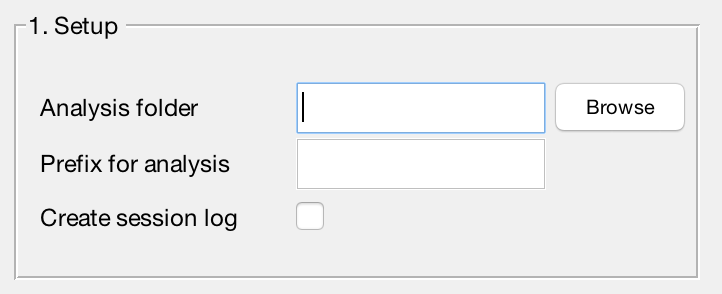
\includegraphics[width=1.2\linewidth]{figs/subpanelsetup}
	\end{column}%
\end{columns}
\end{frame}

\section{Prepare Analysis Panel}

\begin{frame}
\frametitle{Prepare analysis panel}
\begin{columns}[T] % align columns
	\begin{column}{.48\textwidth}
		\color{red}\rule{\linewidth}{0pt}
		
		\begin{itemize}
\item Specify and analysis folder and prefix
\item Load the data and setup the model
\item Preprocess the data
\item Obtain an initial guess for the EM algorithm
\item Remove unwanted independent components from the analysis
\end{itemize}
		
	\end{column}%
	\hfill%
	\begin{column}{.51\textwidth}
		\color{blue}\rule{\linewidth}{0pt}
		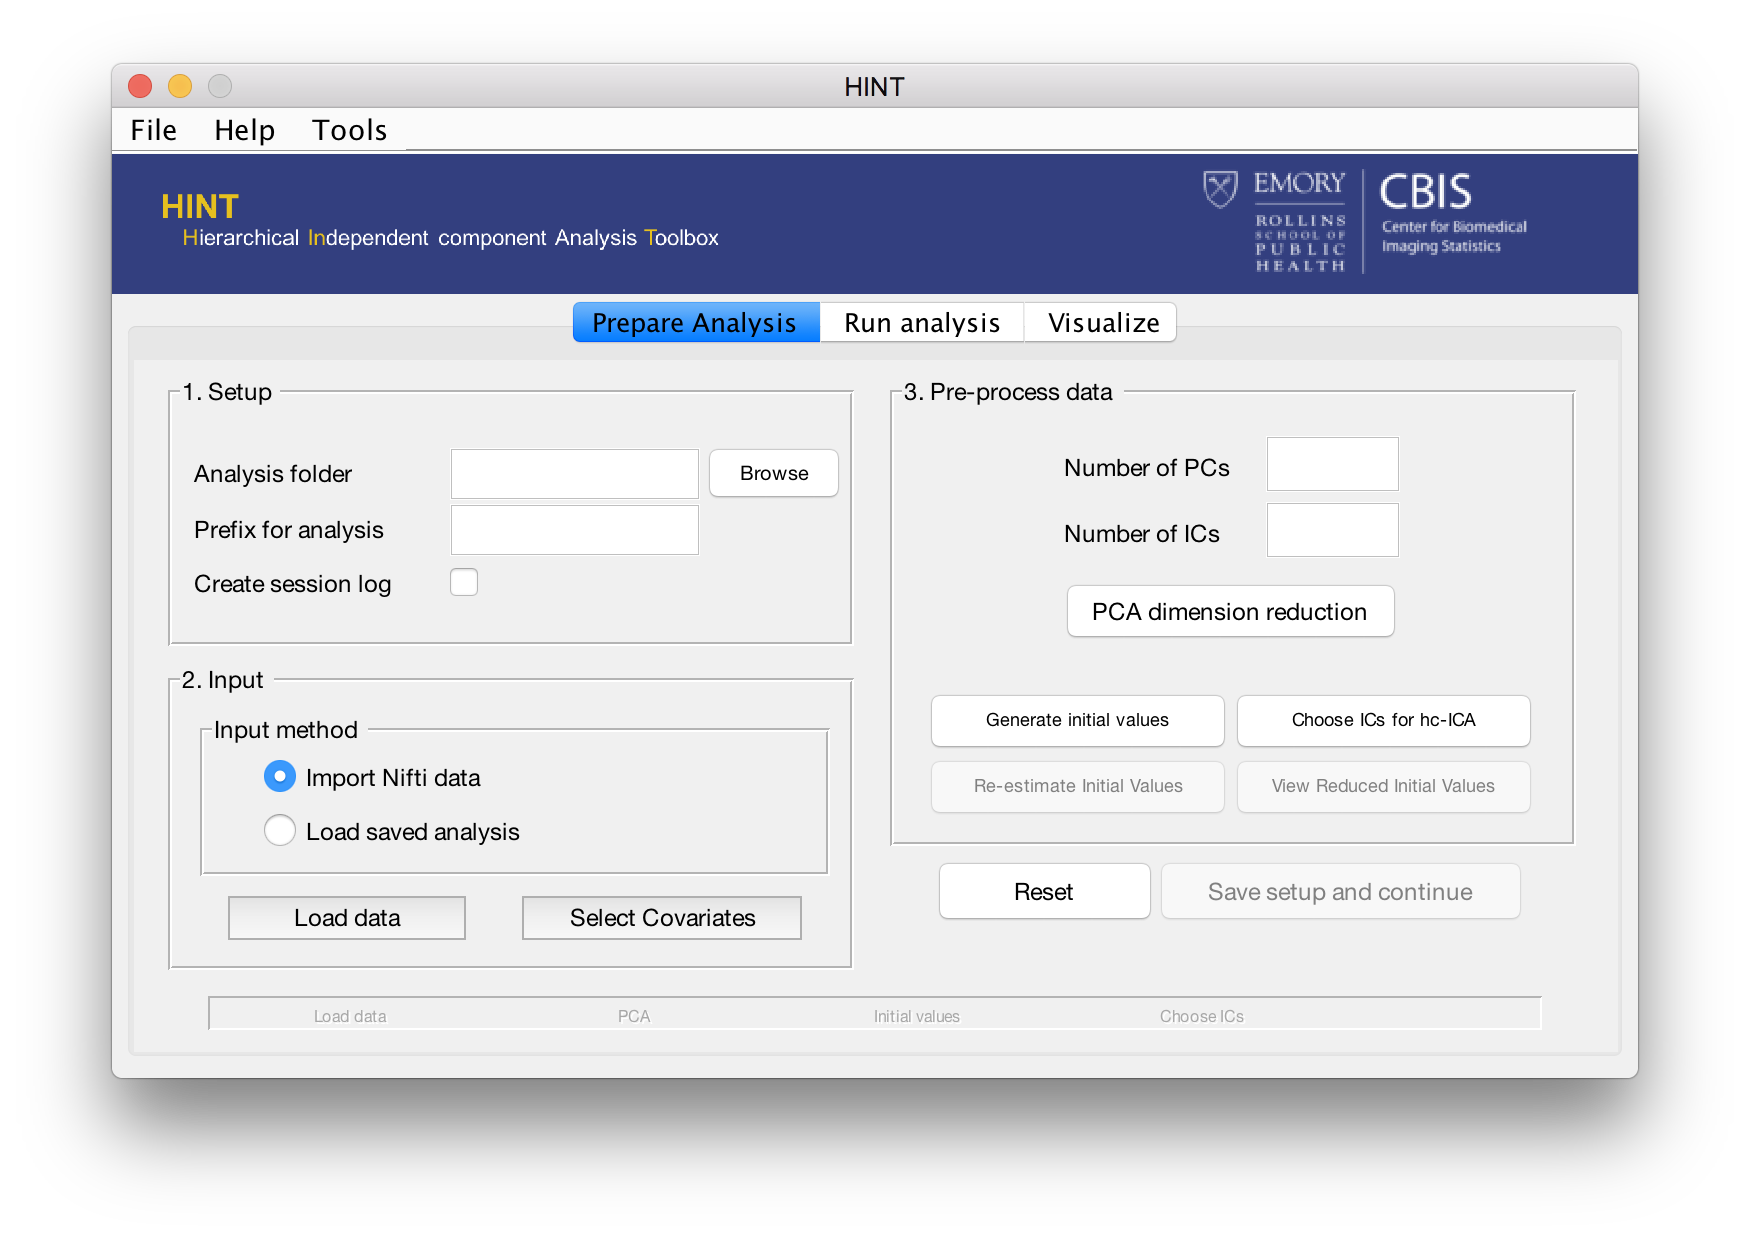
\includegraphics[width=1.2\linewidth]{figs/panel1empty}
	\end{column}%
\end{columns}
\end{frame}

%\begin{frame}{Example Data}
%IN THIS SLIDE FILL OUT THE OUTPUT FOLDER AND THE PREFIX, SHOW EXAMPLE OF OUTPUT FOLDER, SHOW EXAMPLE LOG
%\end{frame}

\subsection{Loading Data}
\begin{frame}{Loading the data}
\begin{columns}[T] % align columns
	\begin{column}{.6\textwidth}
		\color{black}\rule{\linewidth}{0pt}
		
Two options for loading the data

\begin{description}
\item[Import Nifti data] Start a new analysis by selecting the Nifti files, the mask file, and the covariate file.
\item[Load saved analysis] Load a previous HINT analysis by selecting a runinfo file (more on this later).
\end{description}
		
	\end{column}%
	\hfill%
	\begin{column}{.3\textwidth}
		\color{blue}\rule{\linewidth}{0pt}
		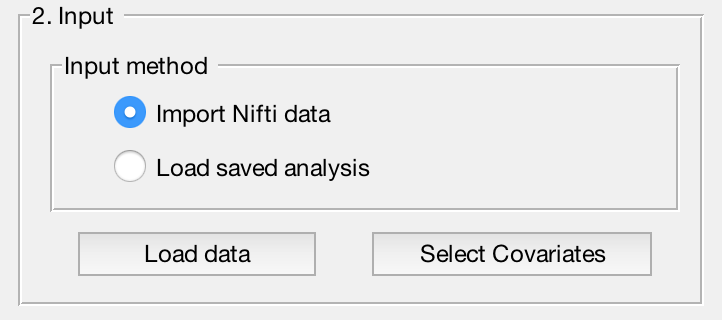
\includegraphics[width=1\linewidth]{figs/subpanelinput}
	\end{column}%
\end{columns}
\end{frame}

\begin{frame}{Loading the data}

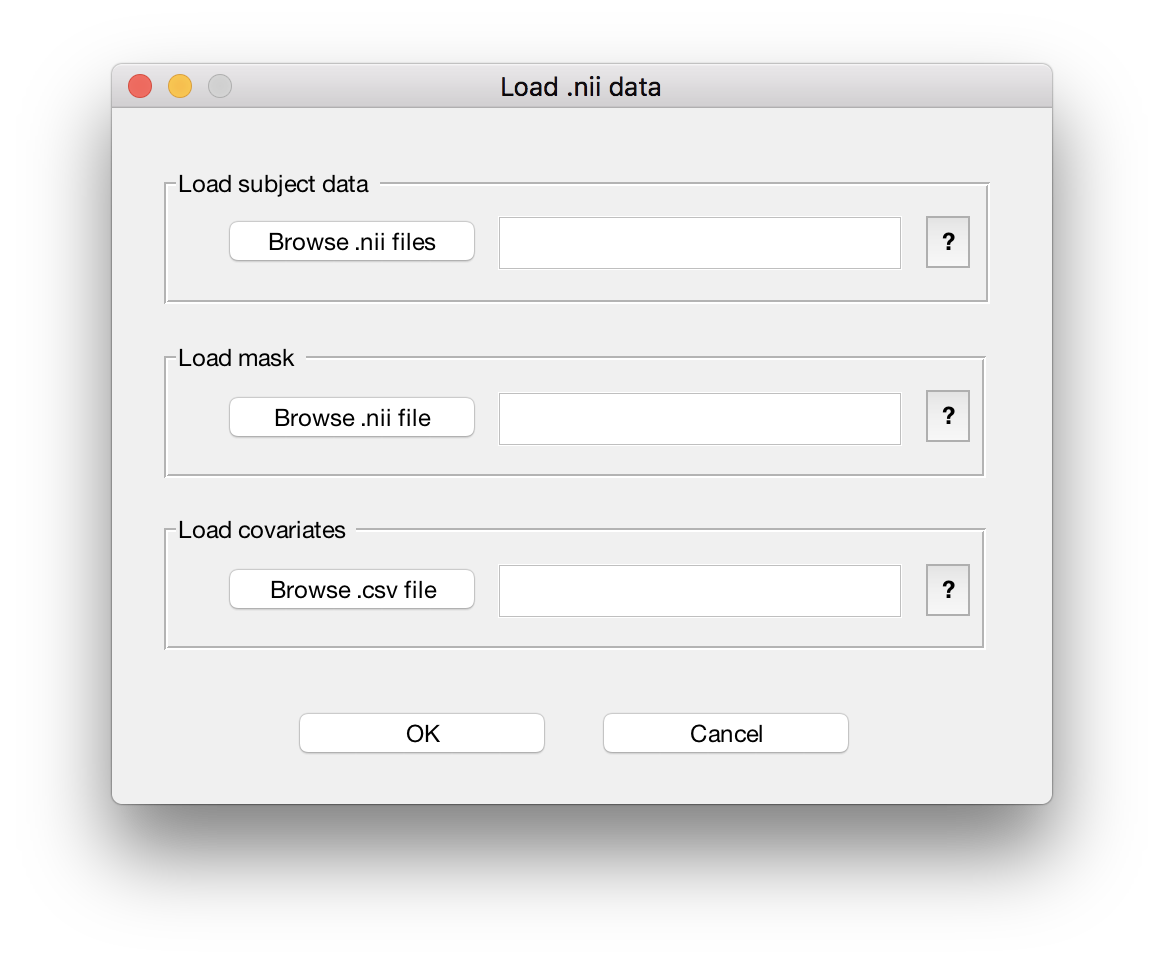
\includegraphics[width=1\linewidth]{figs/inputNIFTI}

\end{frame}

\subsection{Model Specification}
\begin{frame}{Model Specification}
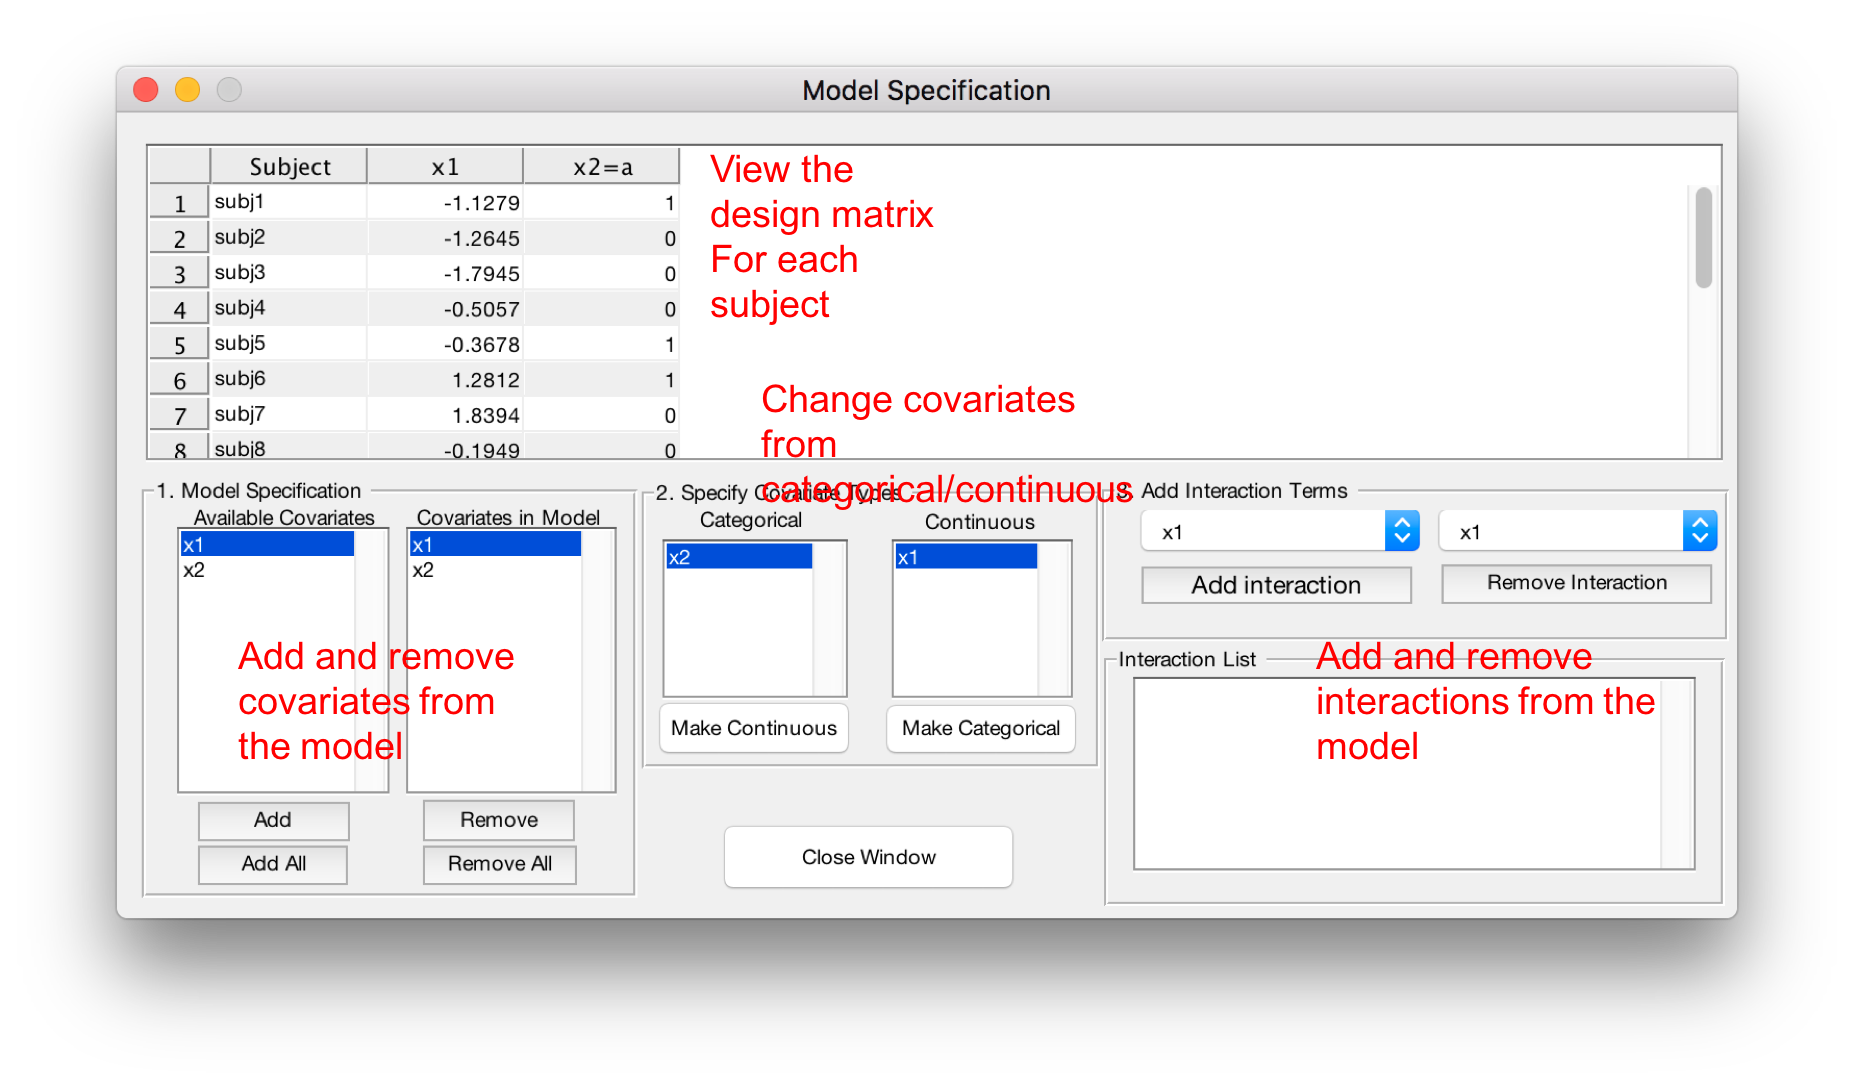
\includegraphics[width=1\linewidth]{figs/covWindowAnnot}
\end{frame}


\subsection{Preprocessing and Initial Guess}

\begin{frame}
\begin{columns}[T] % align columns
	\begin{column}{.6\textwidth}
		\color{black}\rule{\linewidth}{0pt}
		
Analyses in HINT require the data to be demeaned and prewhitened. Two things to select:

\begin{description}
\item[Number of PCs] The number of principal components used by the tc-GICA approach to get an initial guess.
\item[Number of ICs] The number of independent components for the analysis.
\end{description}
		
	\end{column}%
	\hfill%
	\begin{column}{.3\textwidth}
		\color{blue}\rule{\linewidth}{0pt}
		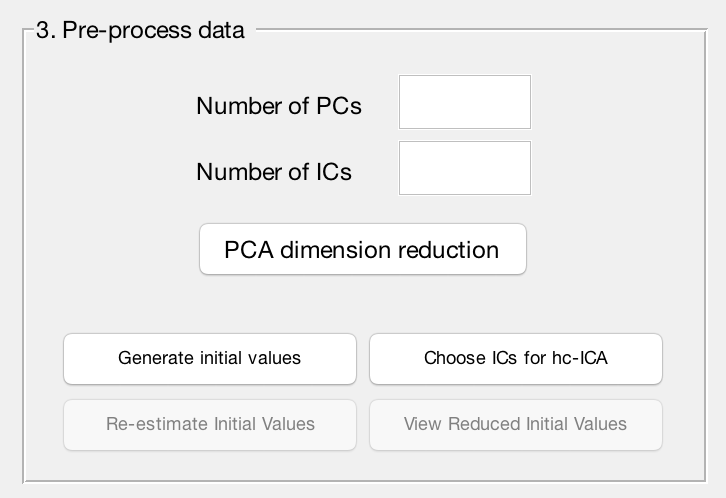
\includegraphics[width=1.2\linewidth]{figs/subpanelpreproc}
	\end{column}%
\end{columns}
\end{frame}

\begin{frame}
After obtaining an initial guess, you will see the following window:
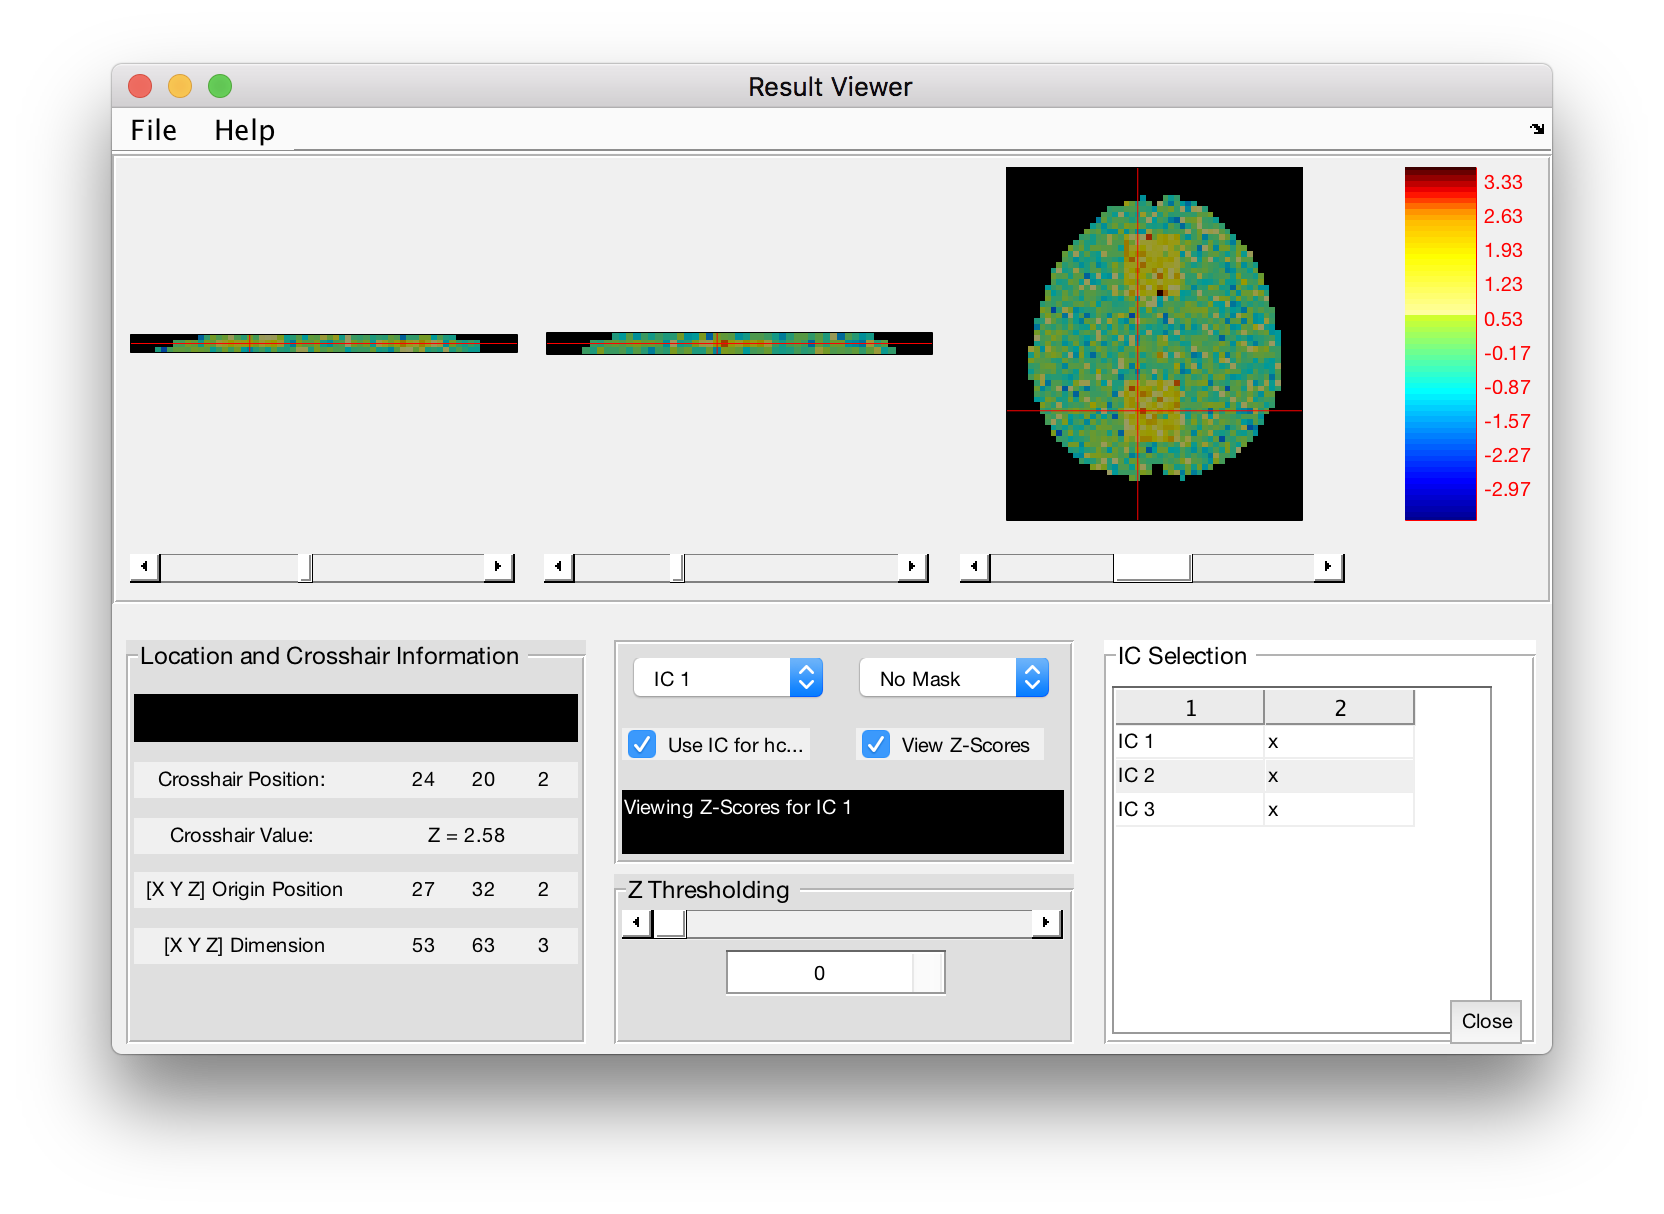
\includegraphics[width=1\linewidth]{figs/iniGuess1}
\end{frame}

\begin{frame}
After verifying that the initial guess looks reasonable, click ``saved setup and continue to move to the second panel. Clicking this also creates a file called the ``runinfo" file in the output directory with all information needed to replicate or change the initial setup.
\end{frame}

\section{Run Analysis Panel}

\begin{frame}
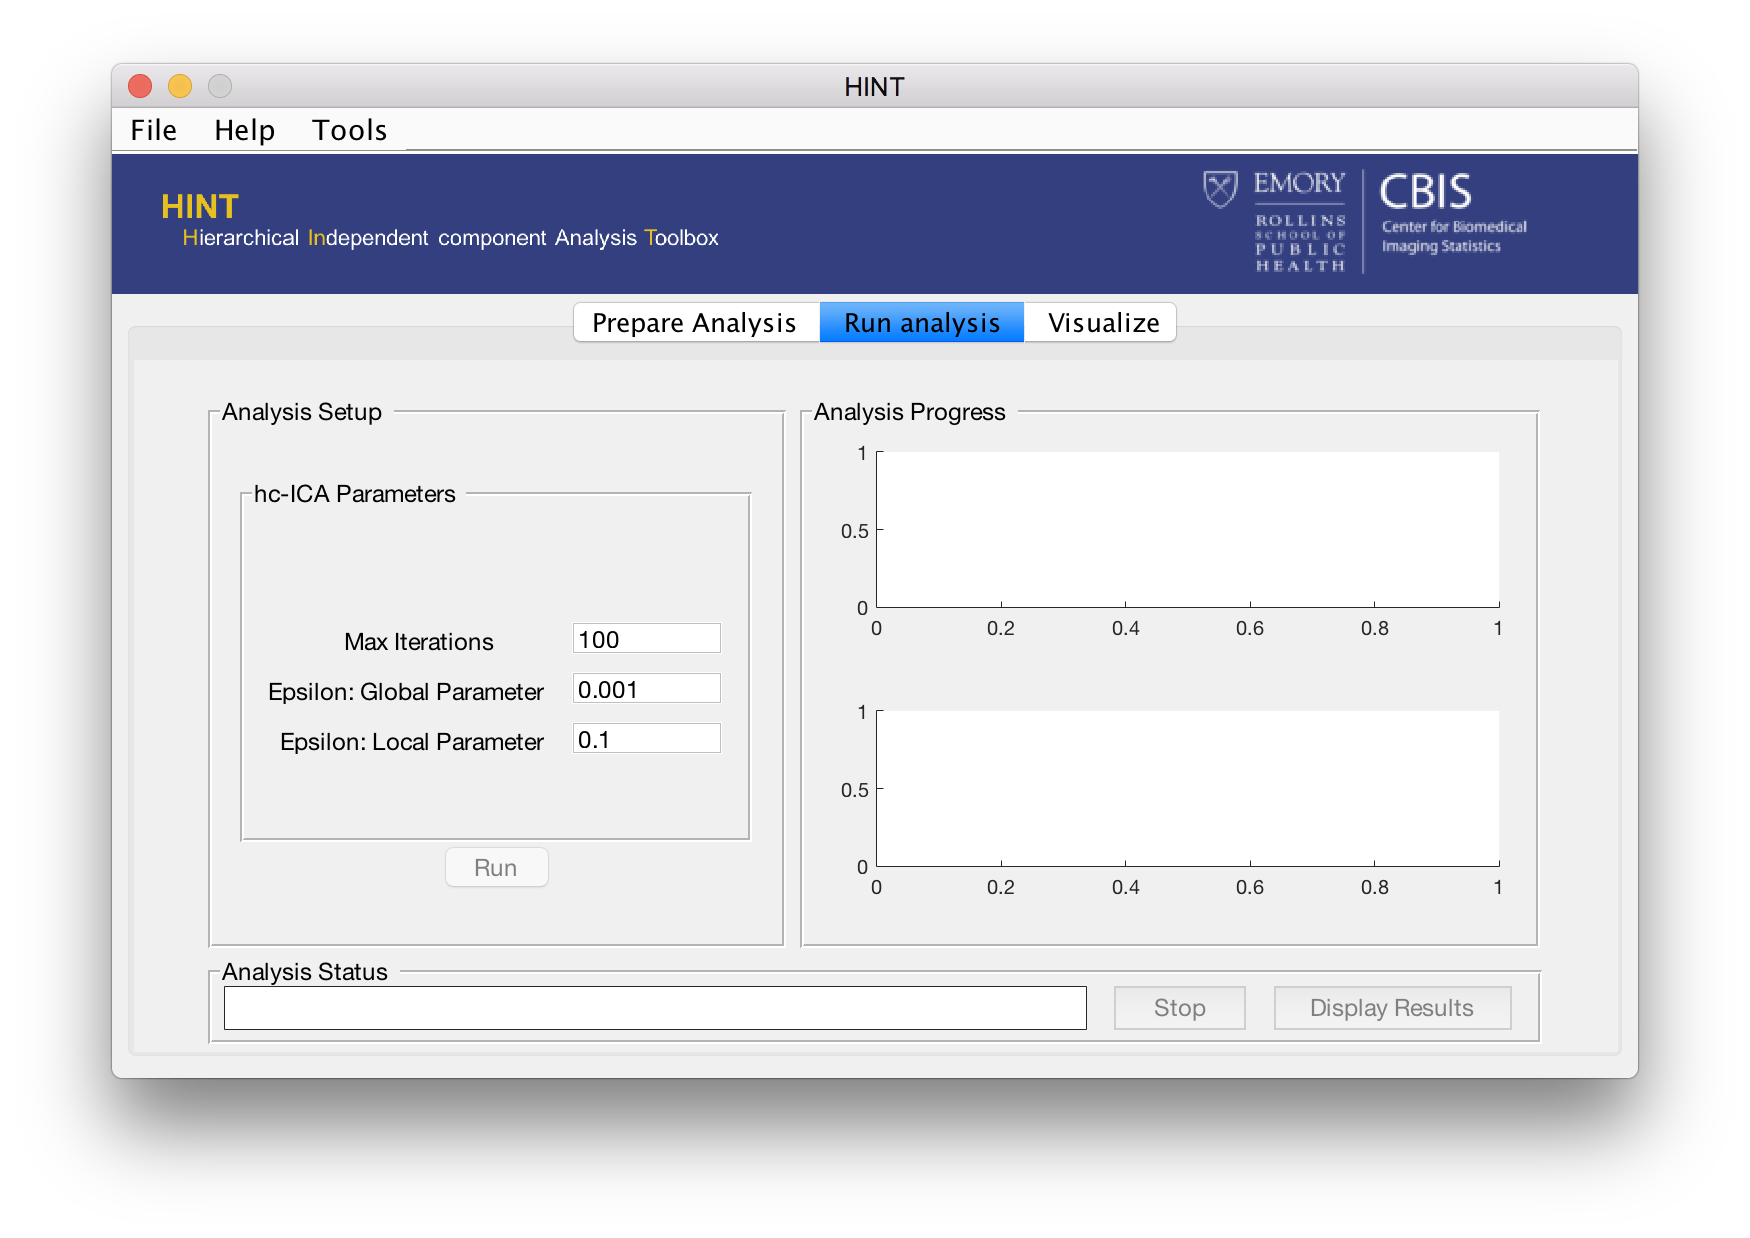
\includegraphics[width=1\linewidth]{figs/panel2empty}
\end{frame}

\begin{frame}
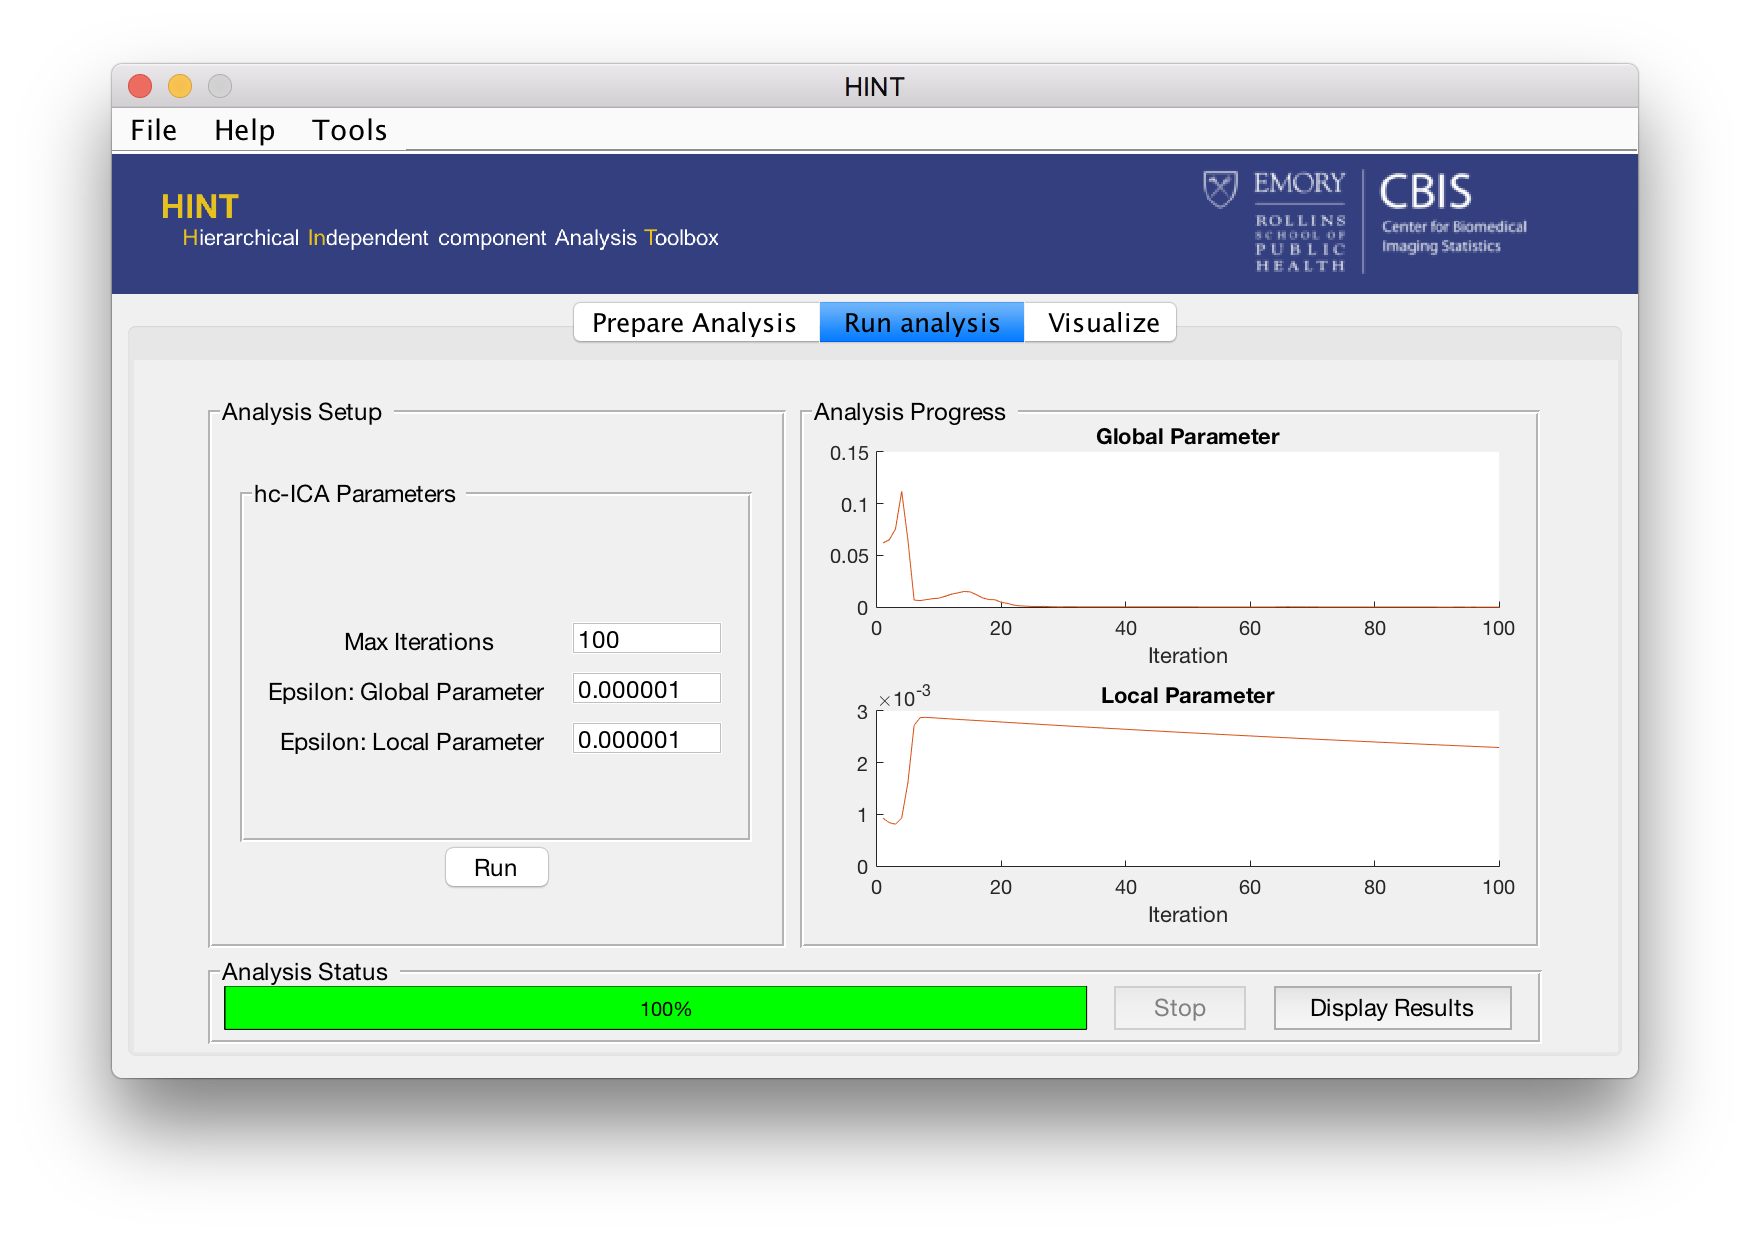
\includegraphics[width=1\linewidth]{figs/panel2filled}
\end{frame}

\section{Visualization Panel}

\begin{frame}
\begin{columns}[T] % align columns
	\begin{column}{.4\textwidth}
		\color{black}\rule{\linewidth}{0pt}
		
\begin{enumerate}
\item Population Level Results
\item Sub-population Level Results
\item Subject Specific Display Maps
\item Beta-coefficient Display Maps
\end{enumerate}
		
	\end{column}%
	\hfill%
	\begin{column}{.6\textwidth}
		\color{blue}\rule{\linewidth}{0pt}
		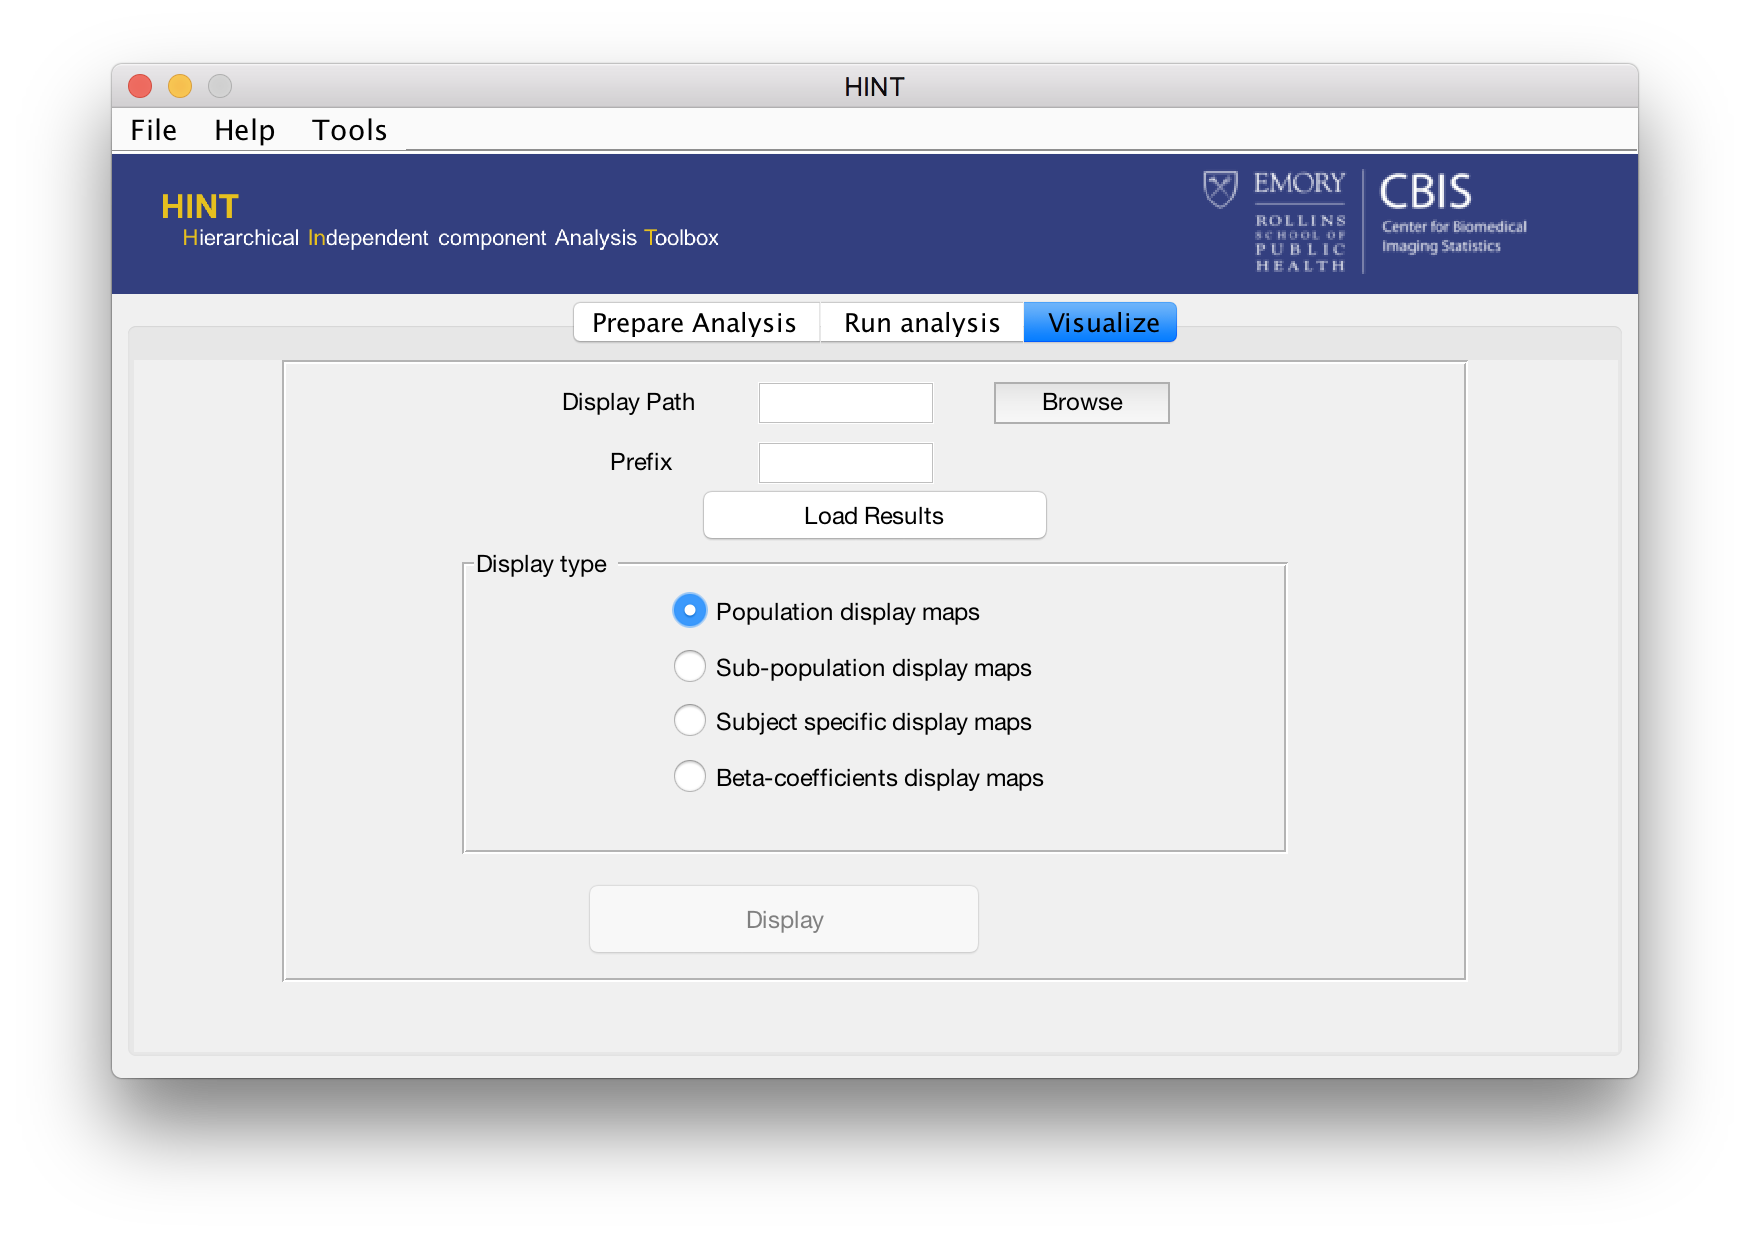
\includegraphics[width=1.2\linewidth]{figs/panel3empty}
	\end{column}%
\end{columns}
\end{frame}

\subsection{Study Population-Level Viewer}

\begin{frame}{Population Level Results}
		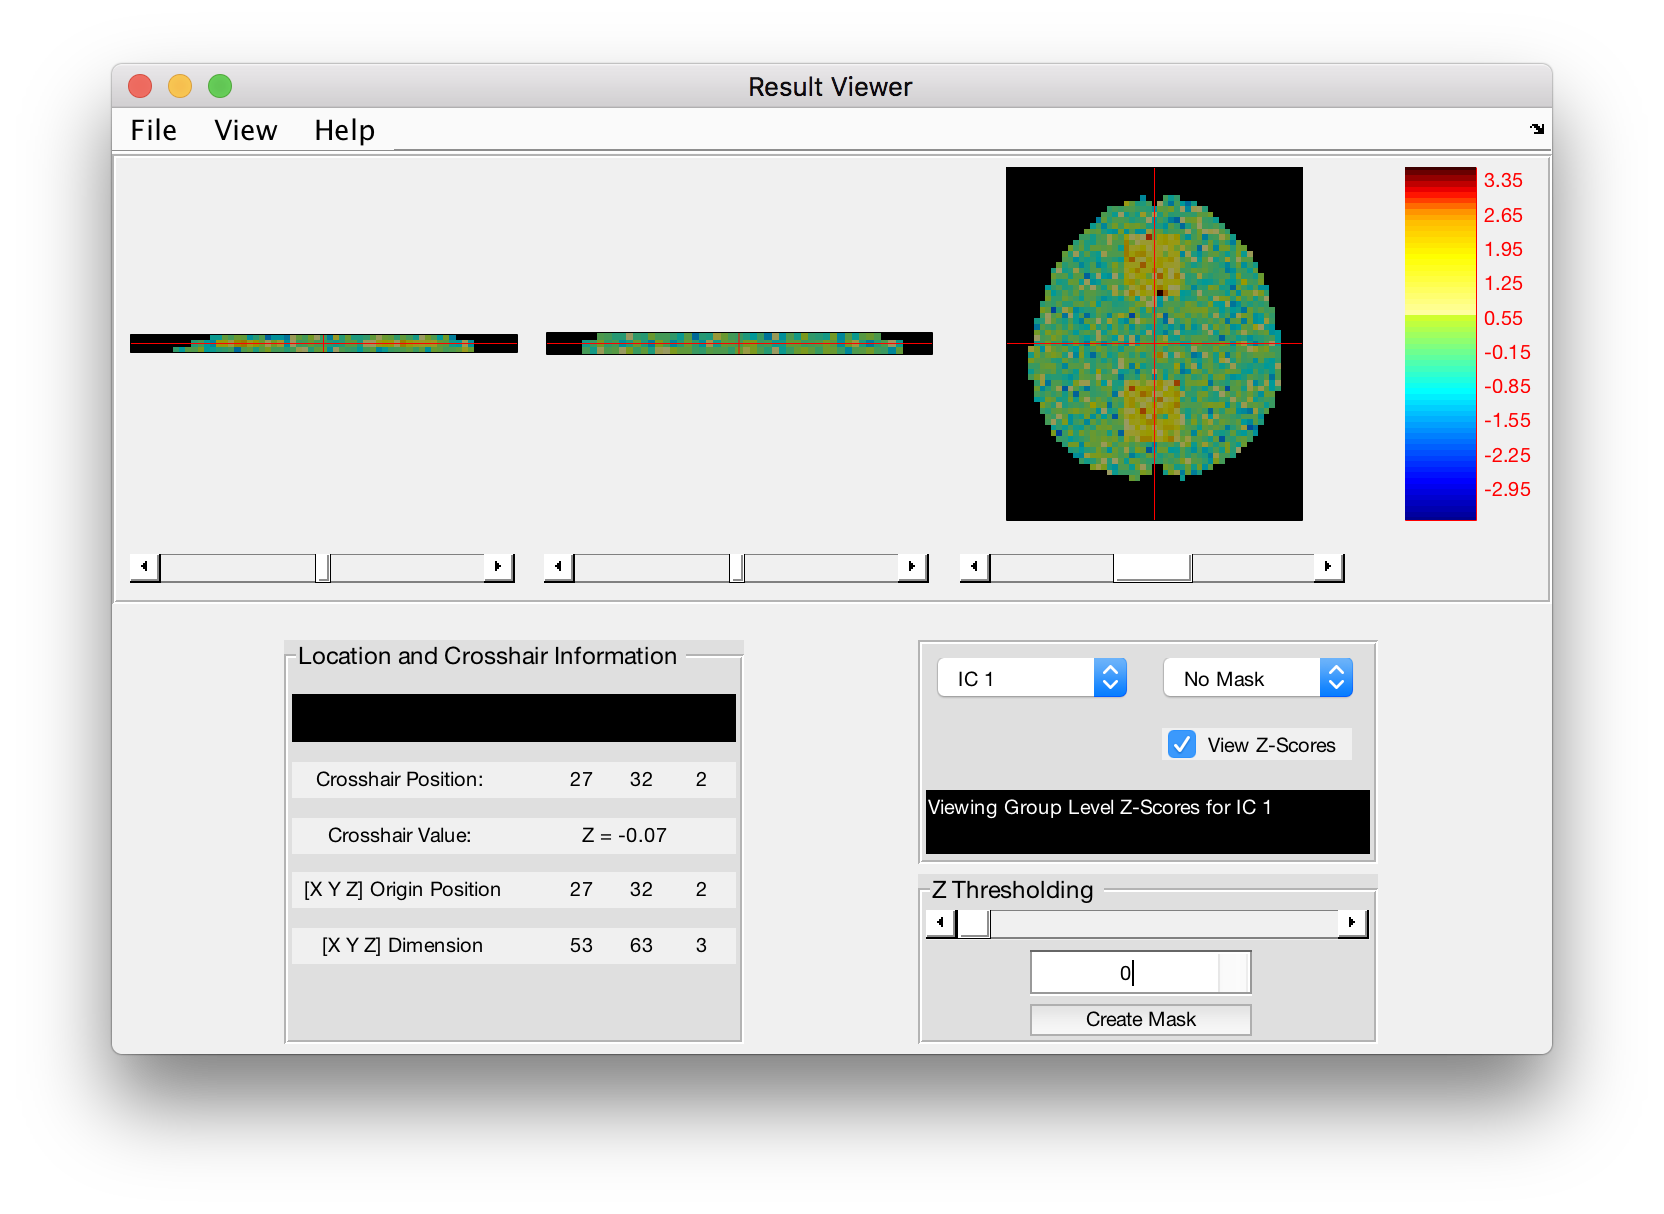
\includegraphics[width=1\linewidth]{figs/viewerPop}
\end{frame}

\begin{frame}{Creating a mask}
		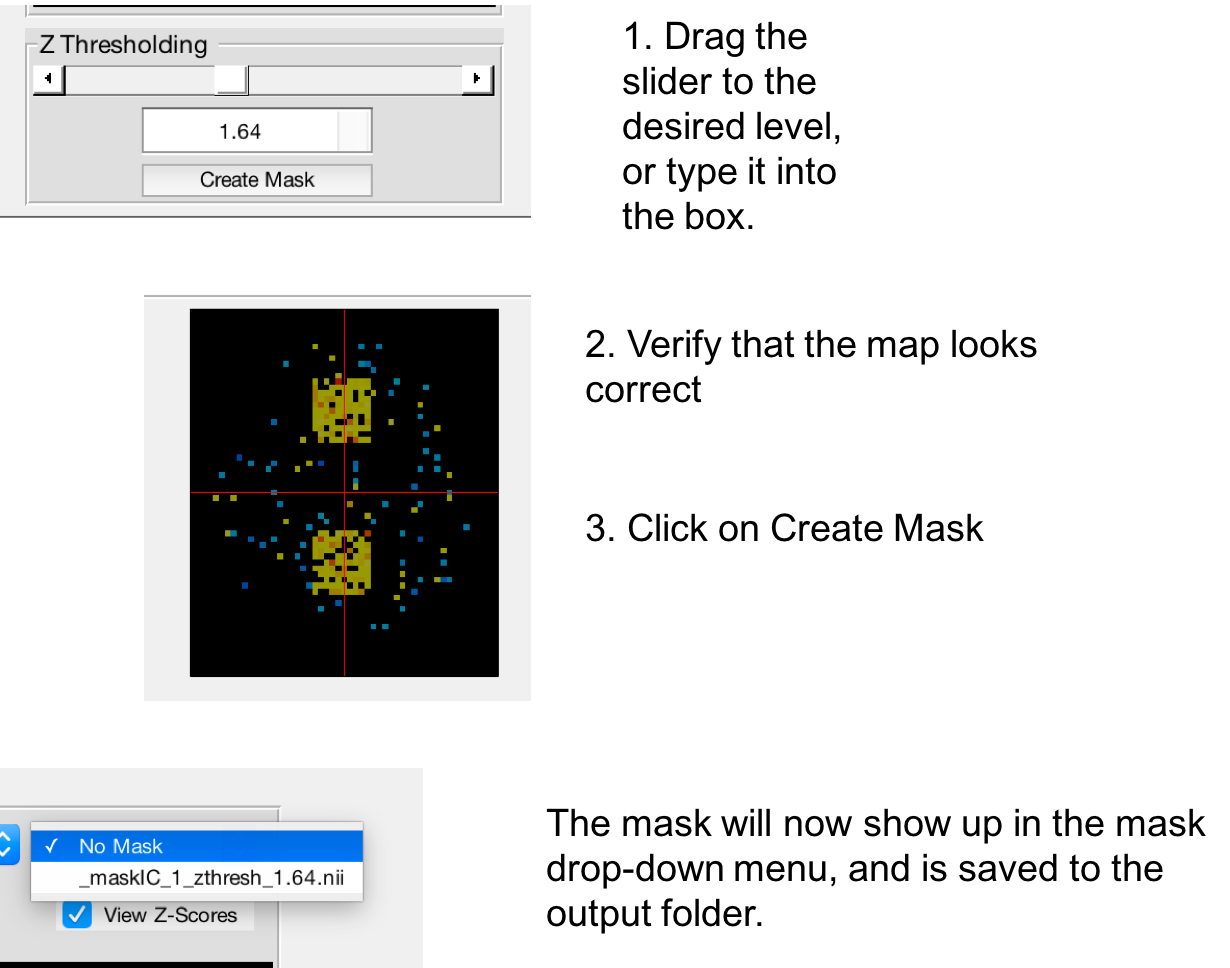
\includegraphics[width=0.8\linewidth]{figs/maskExplanation}
\end{frame}

\subsection{Sub-population Viewer}

\begin{frame}{Sub-population Viewer}
\begin{columns}[T] % align columns
	\begin{column}{.4\textwidth}
		\color{black}\rule{\linewidth}{0pt}

\begin{itemize}	
\item This window allows you to specify sub-populations of interest by entering their covariate values. 
\item Two sub-populations can be compared side-by-side by selecting the ``compare Sub-populations" button.
\end{itemize}
		
	\end{column}%
	\hfill%
	\begin{column}{.6\textwidth}
		\color{blue}\rule{\linewidth}{0pt}
				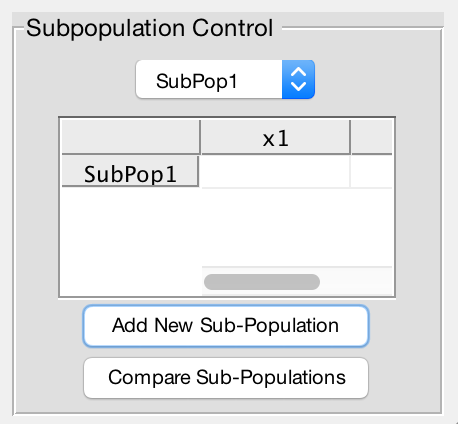
\includegraphics[width=1\linewidth]{figs/viewerSubpopControl}
	\end{column}%
\end{columns}
\end{frame}

\begin{frame}{Comparing Sub-populations}
		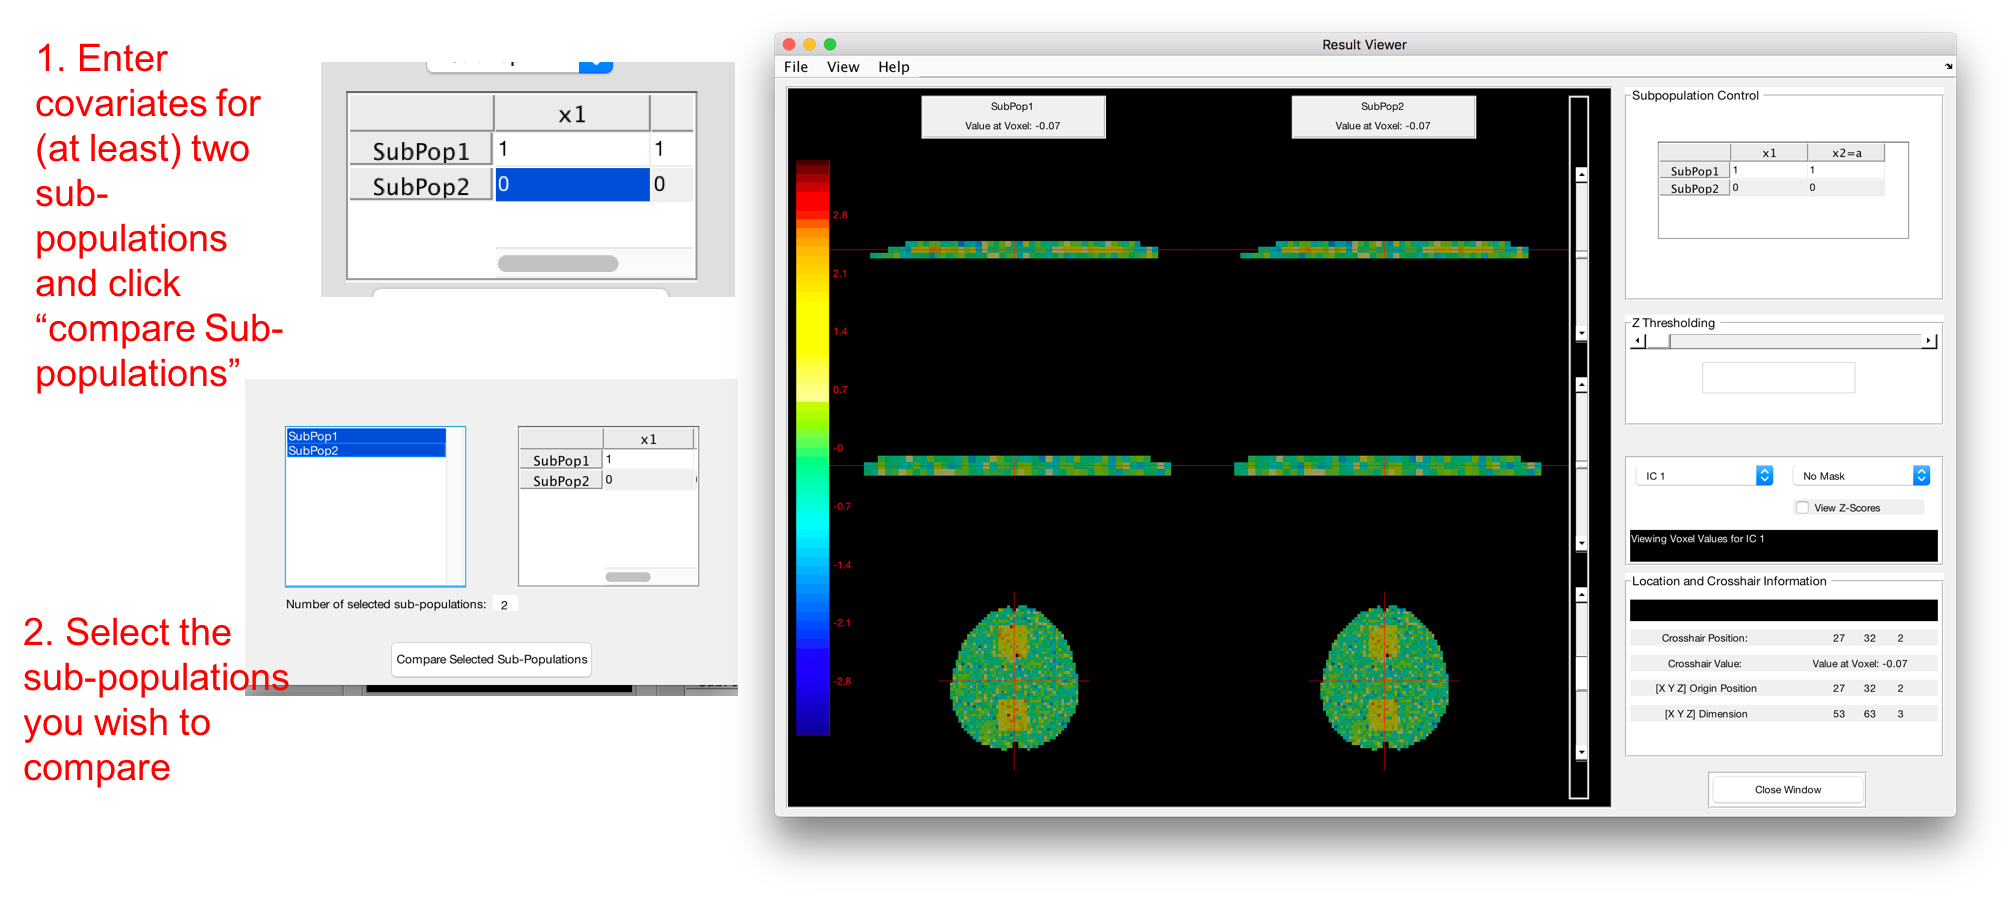
\includegraphics[width=1\linewidth]{figs/subPopCompareEx}
\end{frame}

\subsection{Single Subject Viewer}


\begin{frame}{Single Subject Viewer}
\begin{columns}[T] % align columns
	\begin{column}{.4\textwidth}
		\color{black}\rule{\linewidth}{0pt}

\begin{itemize}	
\item This window allows you to view the IC estimates for individual subjects.
\item You can also apply any mask created using the population-level viewer to the subject level data.
\end{itemize}
		
	\end{column}%
	\hfill%
	\begin{column}{.6\textwidth}
		\color{blue}\rule{\linewidth}{0pt}
				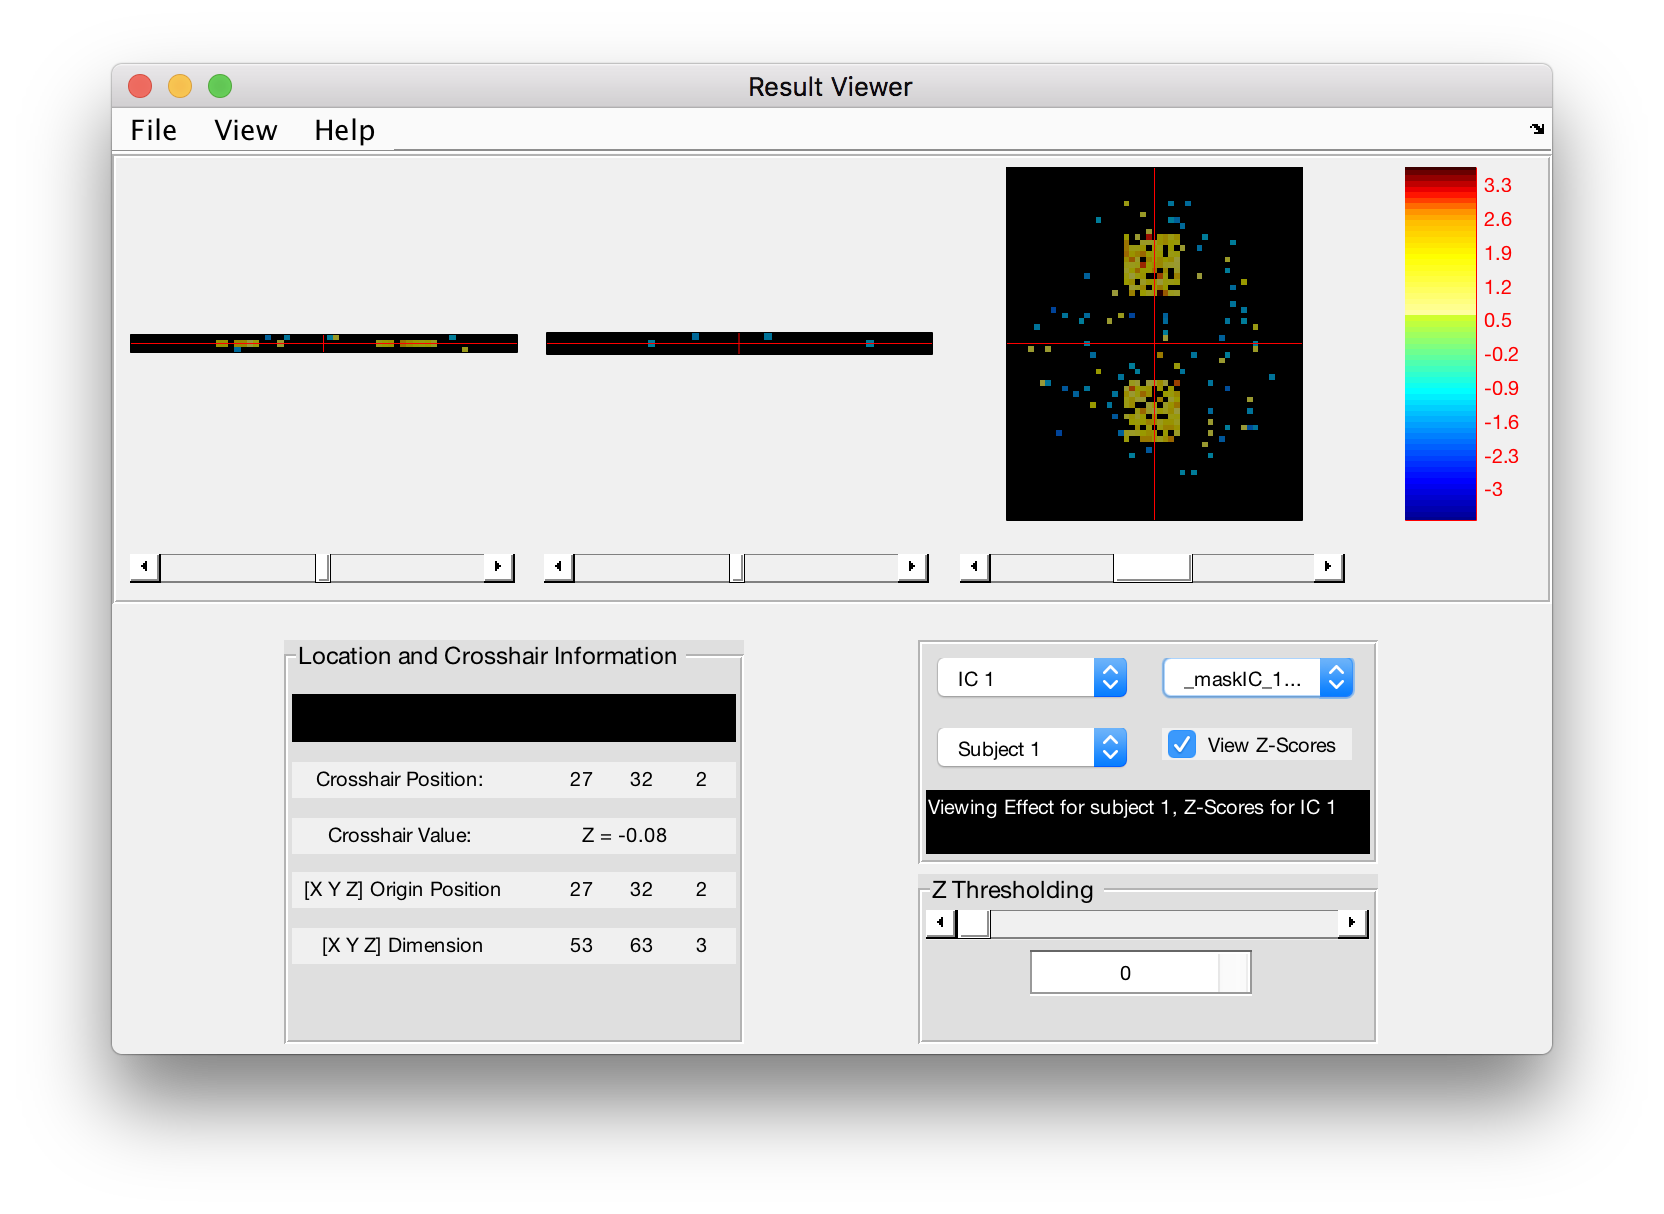
\includegraphics[width=1\linewidth]{figs/singleSubjEx}
	\end{column}%
\end{columns}\end{frame}

\subsection{Beta Coefficient Display Map}

\begin{frame}{Beta Coefficient Display}
		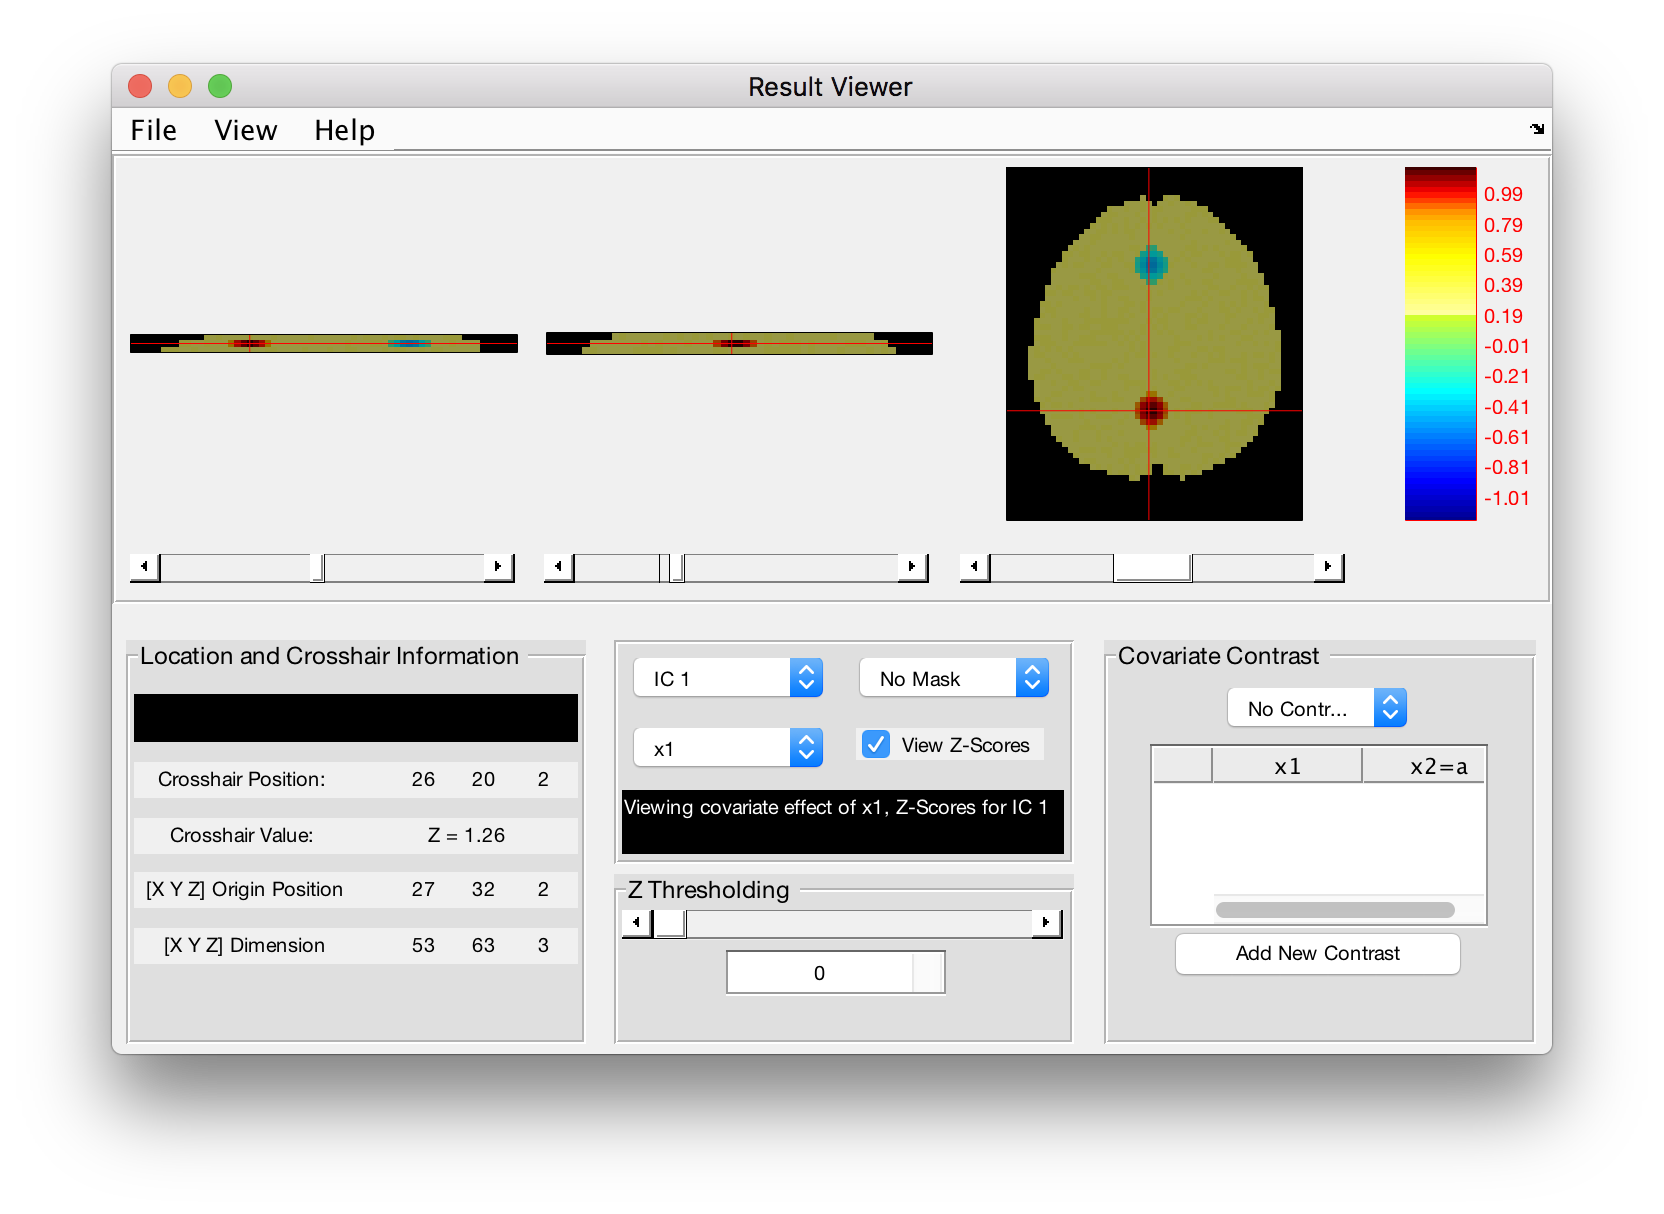
\includegraphics[width=1\linewidth]{figs/betaViewer}
\end{frame}

\begin{frame}{Specifying Contrasts}
		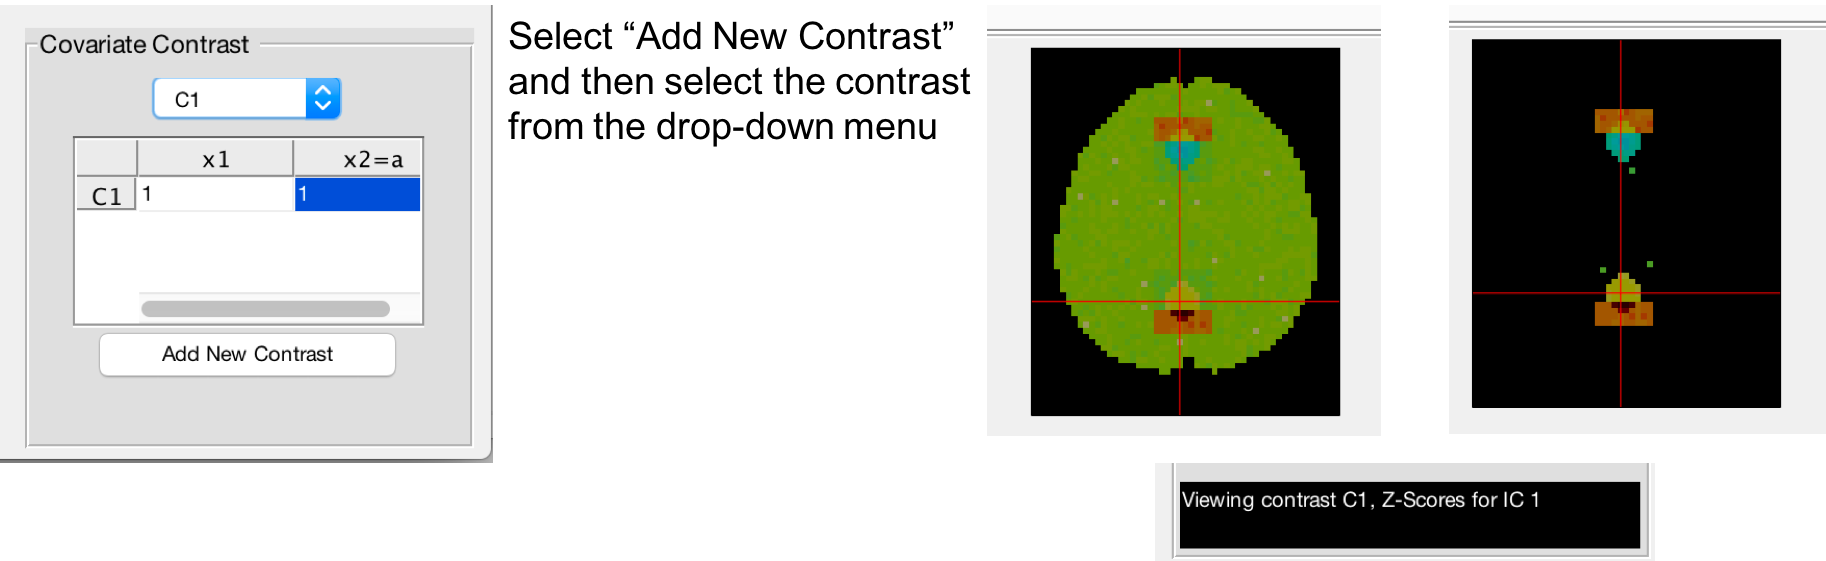
\includegraphics[width=1\linewidth]{figs/contrastExample}
\end{frame}

\section{Other Functionality}

\subsection{Loading a saved analysis}
\begin{frame}{Loading a saved analysis}
Instead of re-starting everything, you can load a previous runinfo file using the ``load a saved analysis" option and navigating to the runinfo file. Everything will auto-fill. However, if you want to re-run the initial guess, you will also have to re-run the preprocessing step. This is for memory reasons.
\end{frame}

\subsection{Removing ICs from the analysis}

\begin{frame}{Removing ICs from the analysis}
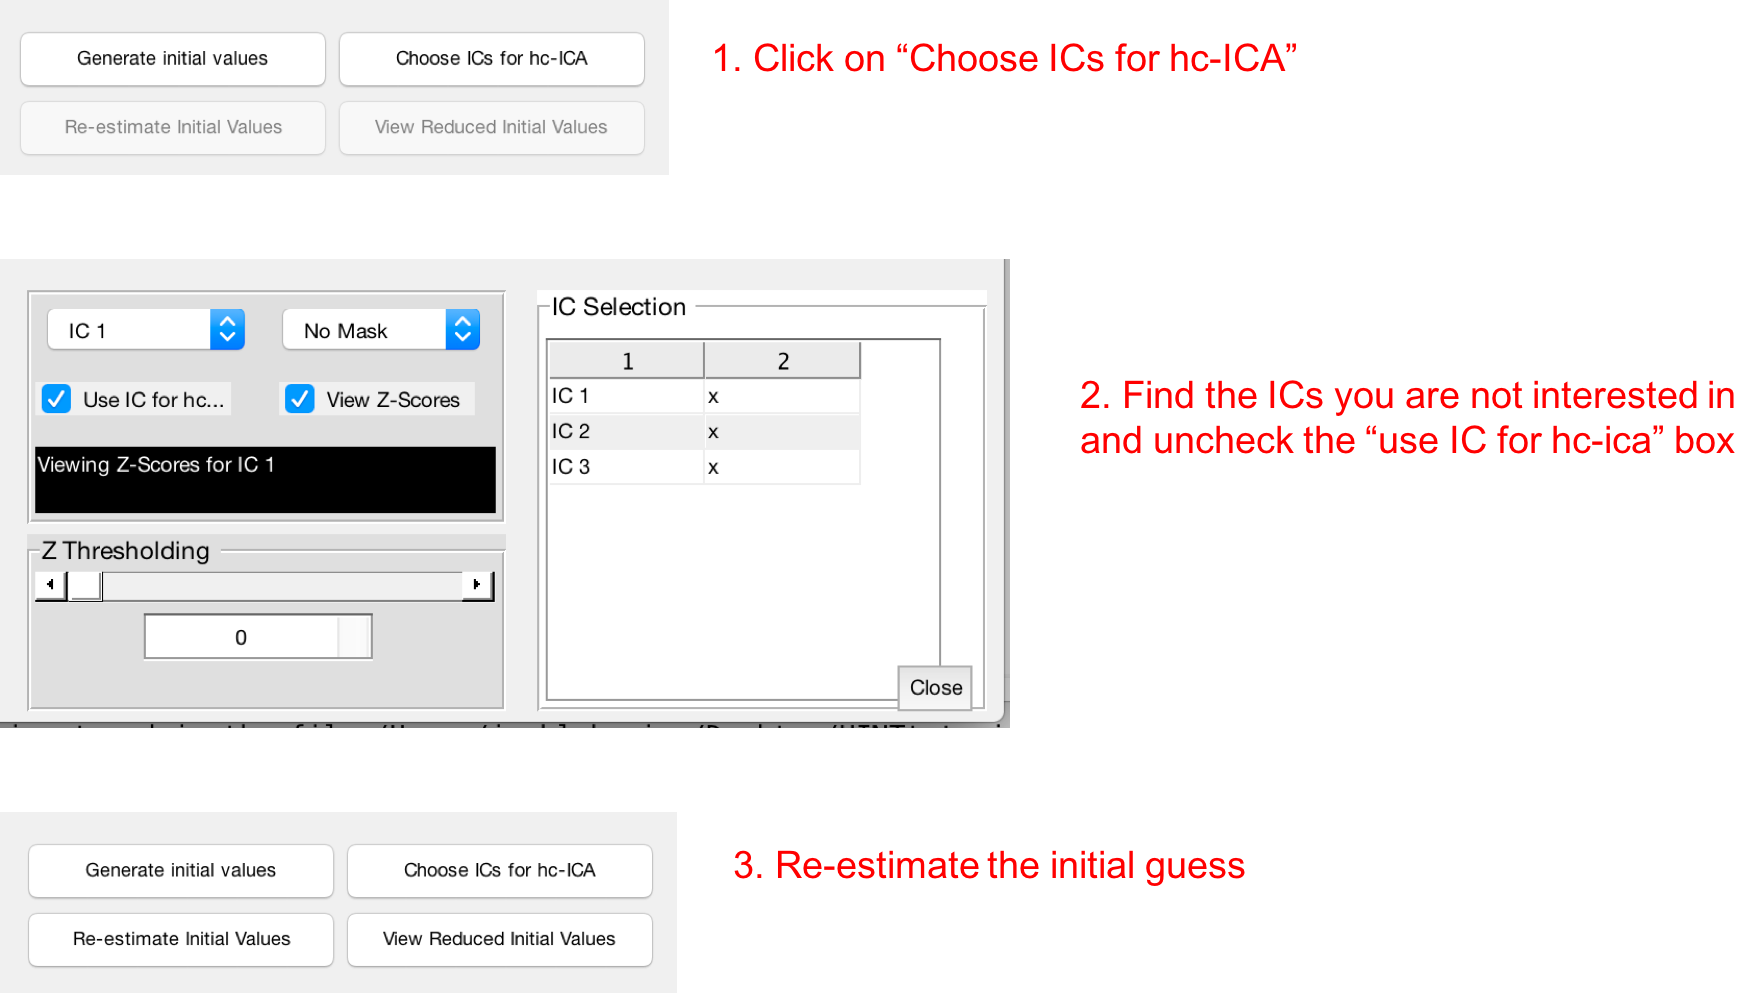
\includegraphics[width=1\linewidth]{figs/removeICex}
 
\end{frame}

\subsection{Running the EM algorithm from a script}
\begin{frame}{Running the EM algorithm from a script}
The matlab function estimateFromSavedData() allows you to run the EM algorithm from a script instead of the GUI. This is used if you want to submit to a cluster instead of running the algorithm on your machine.
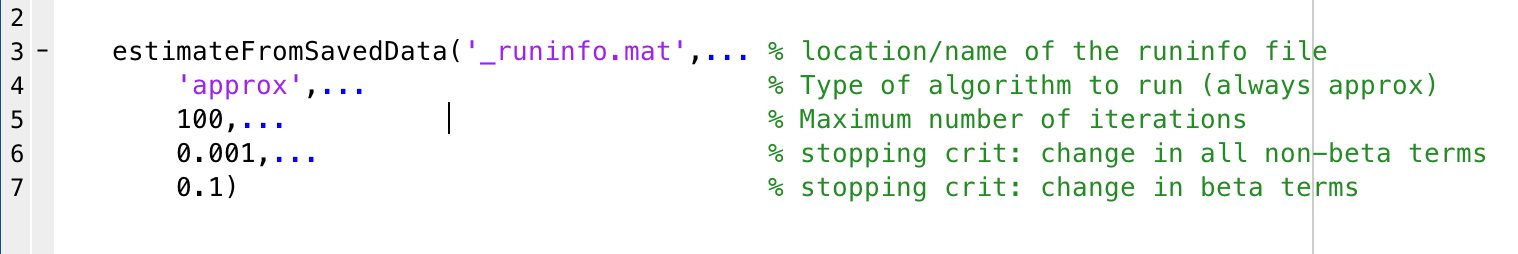
\includegraphics[width=1\linewidth]{figs/scriptVersion}
\end{frame}

\subsection{Compiling iteration results}
\begin{frame}{Compiling iteration results}
If you terminate the EM algorithm early, you may want to use the results from whatever the final completed iteration was. To do this:

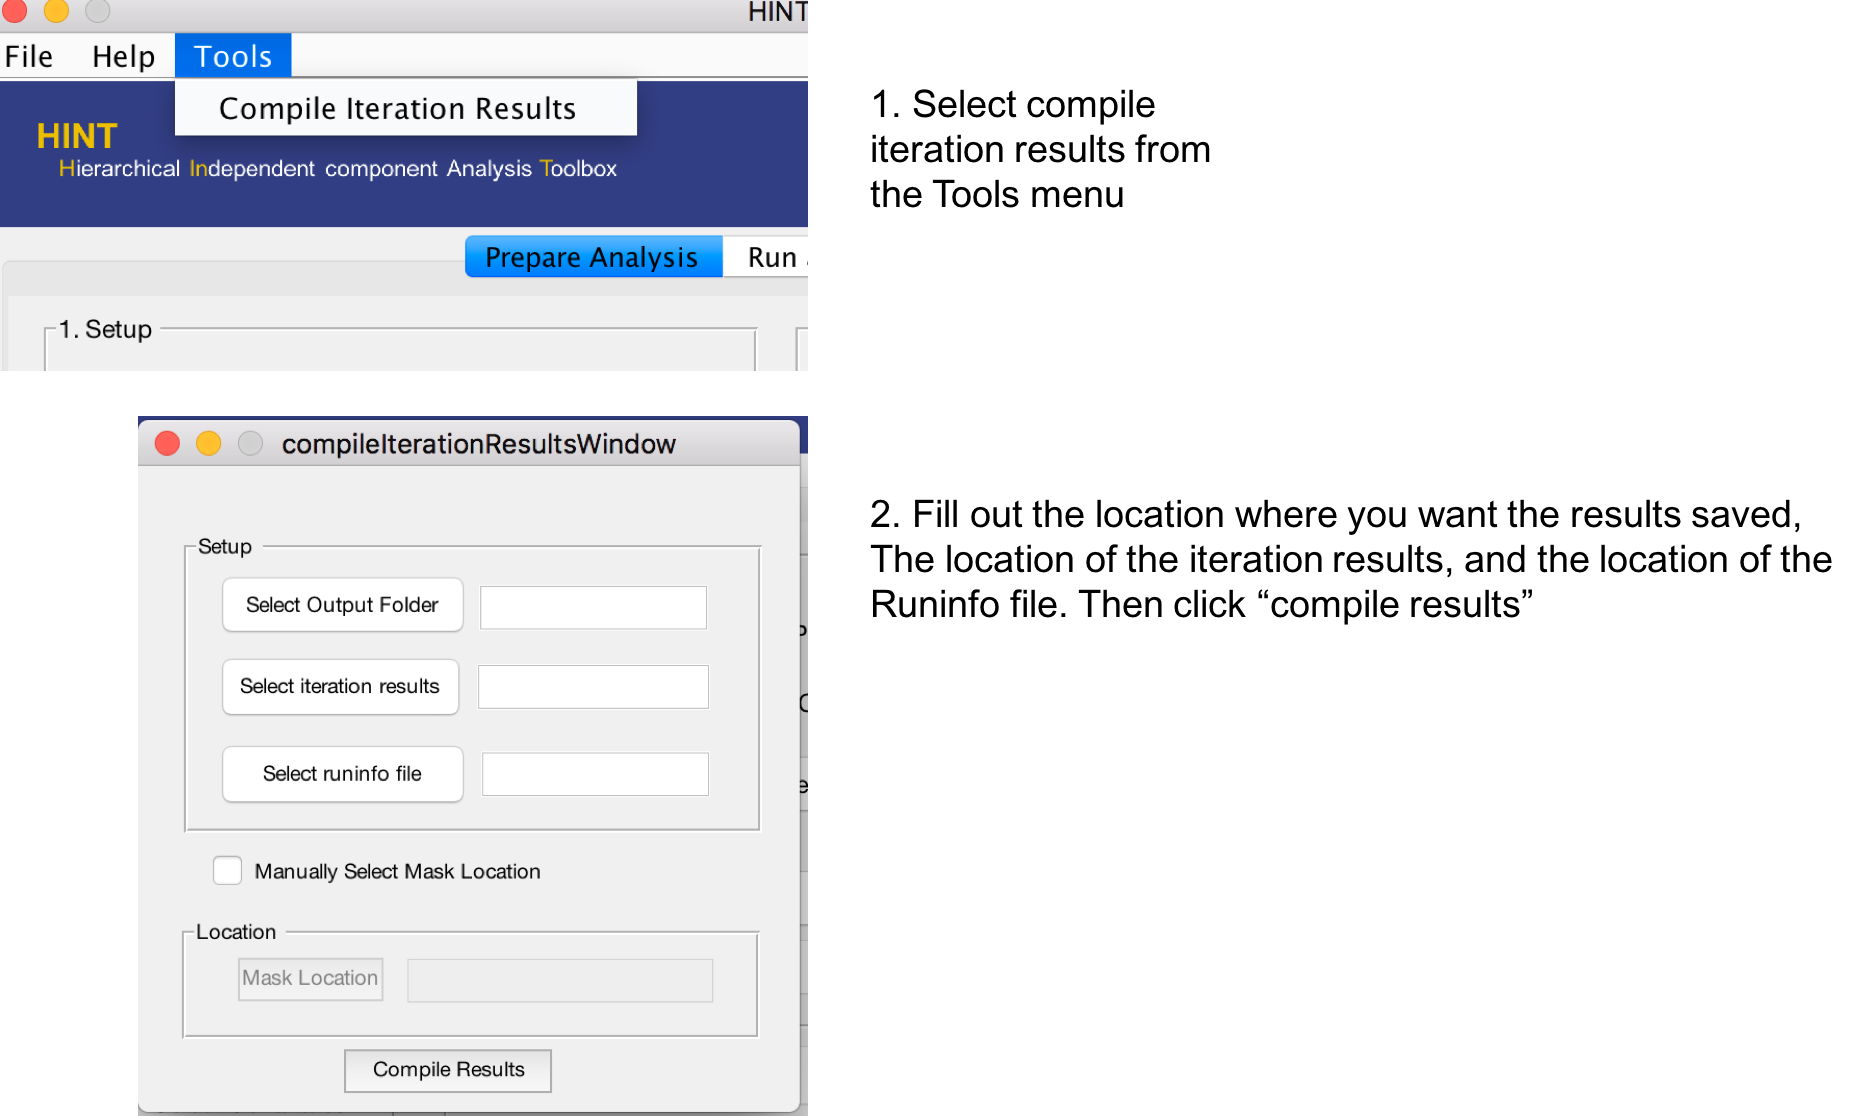
\includegraphics[width=1\linewidth]{figs/compileResultsExample}


\end{frame}



\end{document}